\documentclass[aspectratio=169,usenames,dvipsnames]{beamer}
\usetheme{metropolis}
%\usecolortheme[snowy,cautious]{owl}
\usecolortheme[snowy]{owl}
\metroset{block=fill}

% For regular math font
\usefonttheme[onlymath]{serif}

\usepackage{appendixnumberbeamer}
\usepackage{booktabs}
\usepackage{fancyvrb}
\usepackage{makecell}
\usepackage{xcolor}
%\usepackage{soul}
\usepackage[normalem]{ulem}
\usepackage{hyperref}
\hypersetup{colorlinks,allcolors=.,urlcolor=blue}
\usepackage{graphicx}
\usepackage{siunitx}
\usepackage[siunitx,europeanresistors]{circuitikz}
\usepackage{amsmath}
\usepackage{amssymb}
\usepackage{color}
\usepackage{listings}

% For tikz
\colorlet{darkgreen}{OliveGreen}
\colorlet{darkred}{BrickRed}
% Not used
\definecolor{mygreen}{rgb}{0,0.6,0}
\definecolor{mygray}{rgb}{0.5,0.5,0.5}
\definecolor{mymauve}{rgb}{0.58,0,0.82}
\definecolor{myblue}{rgb}{0,0,1}
% For C
\definecolor{comment}{RGB}{0,128,0} % dark green
\definecolor{string}{RGB}{255,0,0}  % red
\definecolor{keyword}{RGB}{0,0,255} % blue

% Schematic elements colors
\tikzset{
  R/.append style={color=darkred, /tikz/text=black},
  battery1/.append style={color=darkred, /tikz/text=black},
  leDo/.append style={color=darkred, /tikz/text=black},
  short/.append style={color=darkgreen, /tikz/text=black},
  nos/.append style={color=darkred, /tikz/text=black},
  every vcc node/.style={color=darkred, /tikz/text=black},
  every ground node/.style={color=darkred, /tikz/text=black},
  %%% Pin element definition (crossed-out box)
  box/.style={
    rectangle, minimum size=0.5 cm, very thick, draw=black, color=darkred
  },
  pin/.style={
    box,
    append after command={
      [every edge/.append style={
        very thick,
        darkred,
        shorten >=\pgflinewidth,
        shorten <=\pgflinewidth,
      }]
      (\tikzlastnode.north west) edge (\tikzlastnode.south east)
      (\tikzlastnode.north east) edge (\tikzlastnode.south west)
    }
  }
}

% Fix dashs/hyphens in listings
\makeatletter
\lst@CCPutMacro\lst@ProcessOther {"2D}{\lst@ttfamily{-{}}{-{}}}
\@empty\z@\@empty
\makeatother

\newfontfamily\Bera{Bitstream Vera Sans Mono}[Scale=1]
\newfontfamily\TgCursor{TeX Gyre Cursor}[Scale=1]
\newfontfamily\Dejavu{DejaVu Sans Mono}[Scale=1]
%\newfontfamily\Consolas{Consolas}[Scale=0.85]
\newfontfamily\Consolas{Consolas}[Scale=1]

\lstdefinestyle{global} {
%  basicstyle=\fontfamily{cmvtt}\selectfont
%  basicstyle=\tiny\ttfamily,
%  basicstyle=\tiny\Dejavu,
  basicstyle=\tiny\Consolas,
  backgroundcolor=\color{white},
  commentstyle=\itshape\color{comment},
  stringstyle=\color{string},
  keywordstyle=\bfseries\color{keyword},
  %identifierstyle=\bfseries,
  numbers=left,
  numberstyle=\tiny,
  numbersep=5pt,
  frame=lines,
  breaklines=true,
  prebreak=\raisebox{0ex}[0ex][0ex]{\ensuremath{\hookleftarrow}},
  showstringspaces=false,
  upquote=true,
  tabsize=8,
  escapeinside=\`\`,
}

\lstdefinestyle{c} {
  escapeinside=\`\`,
}

\lstdefinestyle{make} {
  language=make,
  morekeywords={if,ifneq,else,elseif,endif},
}

\lstset {
  language=C,
  style=global,
}

% allowframebreaks numbering in the title
\newcounter{cont}
\makeatletter
\setbeamertemplate{frametitle continuation}{%
    \setcounter{cont}{\beamer@endpageofframe}%
    \addtocounter{cont}{1}%
    \addtocounter{cont}{-\beamer@startpageofframe}%
    (\insertcontinuationcount/\arabic{cont})%
}
\makeatother

\title{Kernel Course: Lecture 17}
\subtitle{Communicating with Hardware (part 2)}
\date{\today}
\author{Sam Protsenko}
\institute{GlobalLogic}

\begin{document}

\sisetup{
  math-rm = \mathrm,
  inter-unit-product = \ensuremath{{}\cdot{}},
  per-mode = fraction,
%  fraction-function = \tfrac,
%  unit-color = purple
}

\maketitle

\begin{frame}{Agenda}
  \setbeamertemplate{section in toc}[sections numbered]
  \tableofcontents[hideallsubsections]
\end{frame}

\section{Kernel Driver: Proper Way}

\subsection{API Overview}

\begin{frame}[standout]
  API Overview
\end{frame}

\begin{frame}
  \frametitle{Device/driver matching}
  \begin{itemize}
    \item In real drivers we rarely use just \texttt{module\_init()}
    \item Driver must be platform-independend
    \item Device-specific data is obtained from Device Tree
    \item Driver \textbf{binding} is the process of associating a device with
          a device driver that can control it
    \item Bus drivers (\textit{driver core}) handle this, as bus driver knows
          about all devices and drivers on this bus
  \end{itemize}
\end{frame}

\begin{frame}
  \frametitle{Device/driver matching (cont'd)}
  \begin{itemize}
    \item When driver or device is registered, driver core will check their
          \alert{\texttt{compatible}} strings
    \item If those strings \textbf{match}, driver core will invoke
          \texttt{probe()} function
    \item Platform devices should be registered very early during system boot
    \item Drivers usually register later during booting, or by module loading
  \end{itemize}
  \begin{figure}
    \centering
    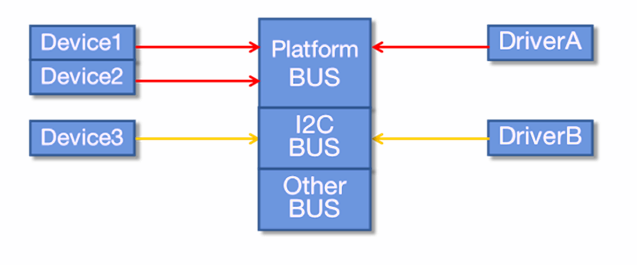
\includegraphics[scale=1.8]{images/platform-bus.png}
  \end{figure}
  \vspace*{-10mm}
\end{frame}

\begin{frame}[containsverbatim]
  \frametitle{API: miscdevice}
  \begin{itemize}
    \item \texttt{miscdevice} = Miscellaneous Character Device
    \item Easier to implement than regular char dev
    \item Major number is the same for all misc devices (see
          \texttt{/proc/devices})
  \end{itemize}

  \begin{lstlisting}[language=c,numbers=none]
#include <linux/miscdevice.h>

struct miscdevice  {
	int minor;
	const char *name;
	const struct file_operations *fops;
	...
};

int misc_register(struct miscdevice *misc);
void misc_deregister(struct miscdevice *misc);
  \end{lstlisting}
\end{frame}

\begin{frame}[containsverbatim]
  \frametitle{API: New GPIO Kernel API}

  \begin{itemize}
  \item Similar set of functions as in ``Legacy GPIO API''
  \item GPIO number is usually obtained from device tree
  \item Operates on \texttt{struct gpio\_desc} (instead of GPIO number)
  \end{itemize}

  \begin{lstlisting}[language=c,numbers=none]
#include <linux/gpio/consumer.h>

/* Get descriptor structure from dts */
struct gpio_desc *__must_check devm_gpiod_get(struct device *dev,
					      const char *con_id,
					      enum gpiod_flags flags);
int gpiod_to_irq(const struct gpio_desc *desc);
void gpiod_set_value(struct gpio_desc *desc, int value);
int gpiod_get_value(const struct gpio_desc *desc);
int gpiod_set_debounce(struct gpio_desc *desc, unsigned debounce); /* usec */
  \end{lstlisting}

  For details see \texttt{Documentation/driver-api/gpio/consumer.rst}.
\end{frame}

\begin{frame}[containsverbatim]
  \frametitle{API: Device Tree}
  \begin{lstlisting}[language=c,numbers=none]
#include <linux/of.h>

/*
 * - can be obtained from struct device (.of_node field), in probe function
 * - contains matched device properties (can be read using functions below)
 */
struct device_node;

/*
 * - to store "compatible" strings table
 * - provide it to struct device (.of_match_table field)
 */
struct of_device_id;

/* Device Tree access functions */
int of_property_read_u32(const struct device_node *np, const char *propname,
			 u32 *out_value);
bool of_property_read_bool(const struct device_node *np, const char *propname);
  \end{lstlisting}

  For details see \texttt{Documentation/devicetree/usage-model.txt}.
  \vspace*{-5mm}
\end{frame}

\begin{frame}[containsverbatim]
  \frametitle{API: Managed Device Resources}

  \begin{itemize}
    \item \texttt{devres} is linked list of memory areas associated with a
          \texttt{struct device}
    \item Each devres entry is associated with a release function
    \item All devres entries are released on driver detach
    \item On release, the associated release function is invoked and then the
devres entry is freed
  \end{itemize}

  \begin{lstlisting}[language=c,numbers=none]
void *devm_kzalloc(struct device *dev, size_t size, gfp_t gfp);
struct gpio_desc *devm_gpiod_get(struct device *dev, const char *con_id,
				 enum gpiod_flags flags);
int devm_request_irq(struct device *dev, unsigned int irq,
		     irq_handler_t handler, unsigned long irqflags,
		     const char *devname, void *dev_id);
  \end{lstlisting}

  For details see \texttt{Documentation/driver-model/devres.txt}.
\end{frame}

\begin{frame}
  \frametitle{Two Flavours of Power Management}

  \begin{block}{Runtime power management (Runtime PM)}
Turn off (stop clock or remove power) hardware components that aren’t
going to be used in the near future, \alert{transparently} from the user space’s
viewpoint.
  \end{block}

  \begin{block}{System sleep}
Knowing in advance that \alert{the whole system} is not going to be used in the
near future, turn off \alert{everything} (possibly \alert{by force}) except for
the RAM chips.
  \end{block}

  \begin{itemize}
  \item We are only going to use \textit{System sleep} PM API
  \item For details see ``System Sleep vs Runtime Power Management'' slides
        (by Rafael J. Wysocki)
  \end{itemize}
\end{frame}

\begin{frame}[containsverbatim]
  \frametitle{API: Power Management}
  \begin{lstlisting}[language=c,numbers=none]
#include <linux/pm.h>

/* Populate it and set to struct driver (.pm field) */
struct dev_pm_ops {
	int (*suspend)(struct device *dev);
	int (*resume)(struct device *dev);
	int (*freeze)(struct device *dev);
	int (*thaw)(struct device *dev);
	int (*poweroff)(struct device *dev);
	int (*restore)(struct device *dev);
};

SIMPLE_DEV_PM_OPS(name, suspend_fn, resume_fn); /* returns struct dev_pm_ops */

int device_init_wakeup(struct device *dev, bool enable);
bool device_may_wakeup(struct device *dev);

int enable_irq_wake(unsigned int irq);
int disable_irq_wake(unsigned int irq);
  \end{lstlisting}
\end{frame}

\subsection{Third Attempt}

\begin{frame}[standout]
  \textbf{Attempt \#3} \\
  \vspace{5mm}
  Platform driver + char dev + new GPIO API + device tree  \\
  \vspace{5mm}
  \textbf{\textcolor{green}{PRODUCTION READY!}}
\end{frame}

\begin{frame}[containsverbatim]
  \frametitle{Third Attempt: Device Tree}
  \lstinputlisting[caption=am335x-boneblack.dts]{materials/module3/dts.txt}
  \vspace*{-5mm}
\end{frame}

\begin{frame}[containsverbatim,allowframebreaks=1]
  \frametitle{Third Attempt: Code}
  \lstinputlisting[caption=hw3.c]{materials/module3/hw3.c}
\end{frame}

\begin{frame}[containsverbatim]
  \frametitle{Third Attempt: Header}
  \lstinputlisting[caption=hw3.h]{materials/module3/hw3.h}
\end{frame}

\begin{frame}[standout]
  Take five
\end{frame}

\section{User space}

\begin{frame}[containsverbatim,allowframebreaks=1]
  \frametitle{User Space Application}
  \lstinputlisting[caption=hw3-app.c]{materials/module3/hw3-app.c}
\end{frame}

\begin{frame}[containsverbatim]
  \frametitle{Makefile}
  \lstinputlisting[caption=Makefile, style=make]{materials/module3/Makefile}
  \vspace*{-5mm}
\end{frame}

\begin{frame}[containsverbatim]
  \frametitle{Building Everything (On Host)}
  Setup environment:
  \begin{lstlisting}[language=bash,numbers=none]
    `\$` export PATH=/opt/gcc-linaro-7.3.1-2018.05-x86_64_arm-linux-gnueabihf/bin:$PATH
    `\$` export CROSS_COMPILE=arm-linux-gnueabihf-
    `\$` export ARCH=arm
    `\$` export KDIR=~/repos/linux-stable
  \end{lstlisting}
  Build new dtb:
  \begin{lstlisting}[language=bash,numbers=none]
    `\$` cd $KDIR
    `\$` make am335x-boneblack.dtb
    `\$` cp arch/arm/boot/dts/am335x-boneblack.dtb $TFTP_DIR
    `\$` cd -
  \end{lstlisting}
  Build module and app:
  \begin{lstlisting}[language=bash,numbers=none]
    `\$` cd $MODULE_DIR
    `\$` make
    `\$` cp hw3.ko hw3-app $NFS_DIR/root
  \end{lstlisting}
\end{frame}

\begin{frame}[containsverbatim]
  \frametitle{Testing Driver From Bash (On Target)}
  \begin{lstlisting}[language=bash,numbers=none]
      `\#` insmod hw3.ko              # load module
      `\#` echo 0 > /dev/hw3          # set LED off
      `\#` echo 1 > /dev/hw3          # set LED on
      `\#` cat /dev/hw3               # poll button

        010010...                  # press Ctrl-C to interrupt

      `\#` rmmod hw3.ko               # unload module
  \end{lstlisting}
  Notice that when driver is in control, LED will toggle on button
  \textbf{press}.
\end{frame}

\begin{frame}[containsverbatim]
  \frametitle{Testing Driver Using App (On Target)}
  \begin{lstlisting}[language=bash,numbers=none]
      `\#` insmod hw3.ko
      `\#` ./hw3-app

        `Waiting for button interrupt [1/20]...`
        `read: 1`
        `Waiting for button interrupt [2/20]...`
        `read: 0`
        `...`

      `\#` rmmod hw3.ko
  \end{lstlisting}
  Notice that when app is in control, LED will toggle on button
  \textbf{release}.
\end{frame}

\begin{frame}[containsverbatim]
  \frametitle{Testing Power Management (On Target)}
  \begin{lstlisting}[language=bash,numbers=none]
      `\#` insmod hw3.ko
      `\#` echo mem > /sys/power/state       # issue suspend

        `PM: suspend entry (deep)`
        `PM: Syncing filesystems ... done.`
        `Freezing user space processes ... (elapsed 0.001 seconds) done.`
        `OOM killer disabled.`
        `Freezing remaining freezable tasks ... (elapsed 0.001 seconds) done.`
        `Suspending console(s) (use no\_console\_suspend to debug)`

        `\textbf{\alert{=== PRESS OUR BUTTON FOR RESUME ===}}`

        `Disabling non-boot CPUs ...`
        `pm33xx pm33xx: PM: Successfully put all powerdomains to target state`
        `OOM killer enabled.`
        `Restarting tasks ... done.`
        `PM: suspend exit`

      `\#` rmmod hw3.ko
  \end{lstlisting}
\end{frame}

\begin{frame}[containsverbatim]
  \frametitle{Kernel Introspection (On Target)}
  \begin{lstlisting}[language=bash,numbers=none]
`\#` cat /proc/interrupts | grep hw3
`63:         \textbf{18}  44e07000.gpio  27 Edge      hw3`

`\#` cat /sys/kernel/debug/gpio
`gpiochip0: GPIOs 0-31, parent: platform/44e07000.gpio, gpio-0-31:`
` gpio-27  (                    |button              ) in  hi IRQ`
`gpiochip1: GPIOs 32-63, parent: platform/4804c000.gpio, gpio-32-63:`
` gpio-47  (                    |led                 ) out hi`

`\#` find /sys/kernel/debug/pinctrl/ -exec grep -Hn hw3 {} \;
`...`

`\#` ls -1 /sys/firmware/devicetree/base/hw3/
`button-gpios`
`compatible`
`debounce-delay-ms`
`led-gpios`
`wakeup-source`
`...`

`\#` cat /sys/firmware/devicetree/base/hw3/debounce-delay-ms | hexdump
  \end{lstlisting}
  \vspace*{-10mm}
\end{frame}

\section{Assignments}

\begin{frame}
  \frametitle{Assignment 1}
  \begin{itemize}
    \item Assemble LED + button device on the breadboard
    \item Build \texttt{hw3.ko}, \texttt{hw3-app} and modified
          \texttt{am335x-boneblack.dtb}
    \item Boot kernel with new \texttt{dtb} and load \texttt{hw3.ko}
    \item Test it with Bash commands
    \item Test it with \texttt{hw3-app}
    \item Inspect \texttt{hw3.ko} driver using kernel introspection capabilities
    \item Make sure you are using NFS for development
    \item Make sure you are able to jump between both kernel functions and
          your driver code functions
  \end{itemize}
\end{frame}

\begin{frame}
  \frametitle{Assignment 2}
  \begin{itemize}
    \item Connect matrix keypad to BBB (directly or using breadboard)
    \item Implement driver for detecting pressed buttons
    \item Report detected buttons to kernel log (\texttt{dmesg})
    \item Use work queue for scanning columns
    \item Obtain scan interval from device tree definition
    \item Perform reading rows on interrupt
    \item Configure debouncing for rows lines
    \item Use platform driver and device tree
  \end{itemize}
\end{frame}

\begin{frame}
  \frametitle{Assignment 2 (cont'd)}
  \begin{columns}
    \column{0.5\textwidth}
      \begin{figure}
        \centering
        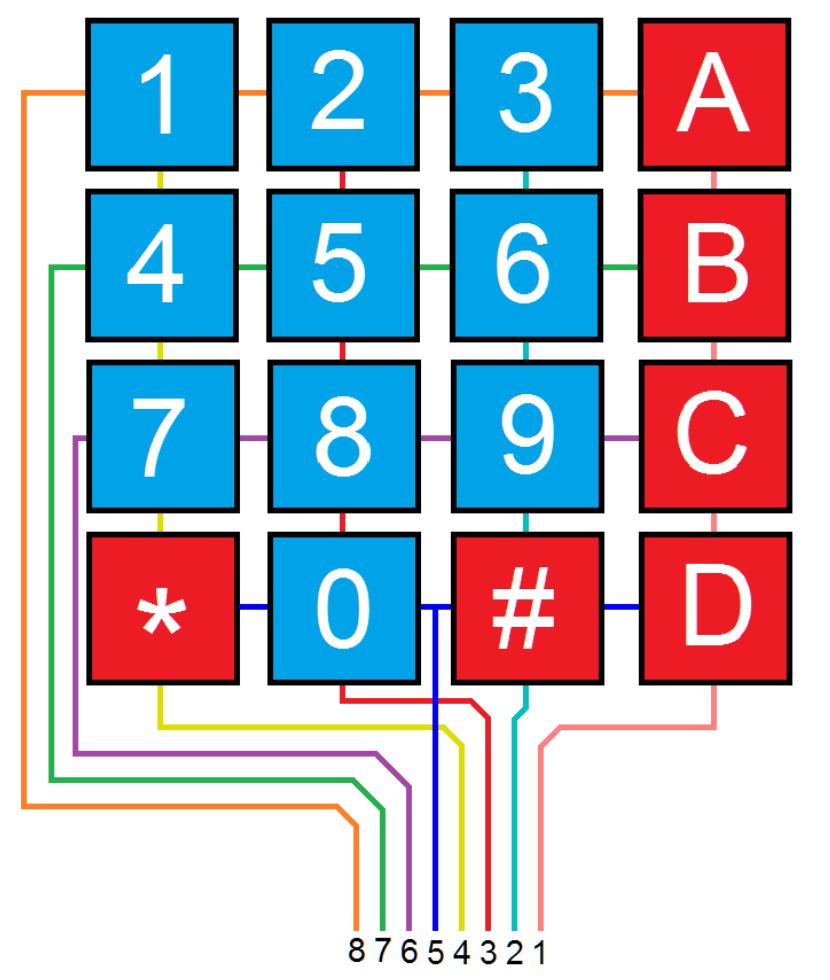
\includegraphics[scale=0.2]{images/keypad-pinout1.png}
      \end{figure}
    \column{0.5\textwidth}
      \begin{figure}
        \centering
        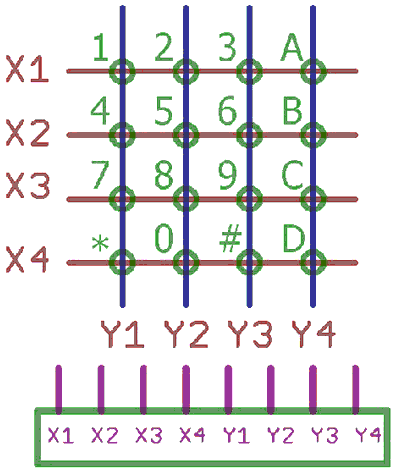
\includegraphics[scale=0.4]{images/keypad-pinout2.png}
      \end{figure}
  \end{columns}
\end{frame}

\begin{frame}
  \frametitle{Assignment 2 (cont'd)}
      \begin{table}
        \begin{tabular}{| l | l | l |}
          \toprule
          GPIO line & Pin name & BBB pin      \\
          \midrule
          gpio0\_26 & gpmc\_ad10 & P8.14      \\
          gpio0\_27 & gpmc\_ad11 & P8.17      \\
          gpio1\_12 & gpmc\_ad12 & P8.12      \\
          gpio1\_13 & gpmc\_ad13 & P8.11      \\
          gpio1\_14 & gpmc\_ad14 & P8.16      \\
          gpio1\_15 & gpmc\_ad15 & P8.15      \\
          gpio1\_17 & gpmc\_a1   & P9.23      \\
          gpio1\_29 & gpmc\_csn0 & P8.26      \\
          \bottomrule
        \end{tabular}
      \end{table}
\end{frame}

\begin{frame}
  \frametitle{Assignment 2 (cont'd)}
  \vspace*{-5mm}
  \begin{columns}
    \column{0.6\textwidth}
      \begin{figure}
        \centering
        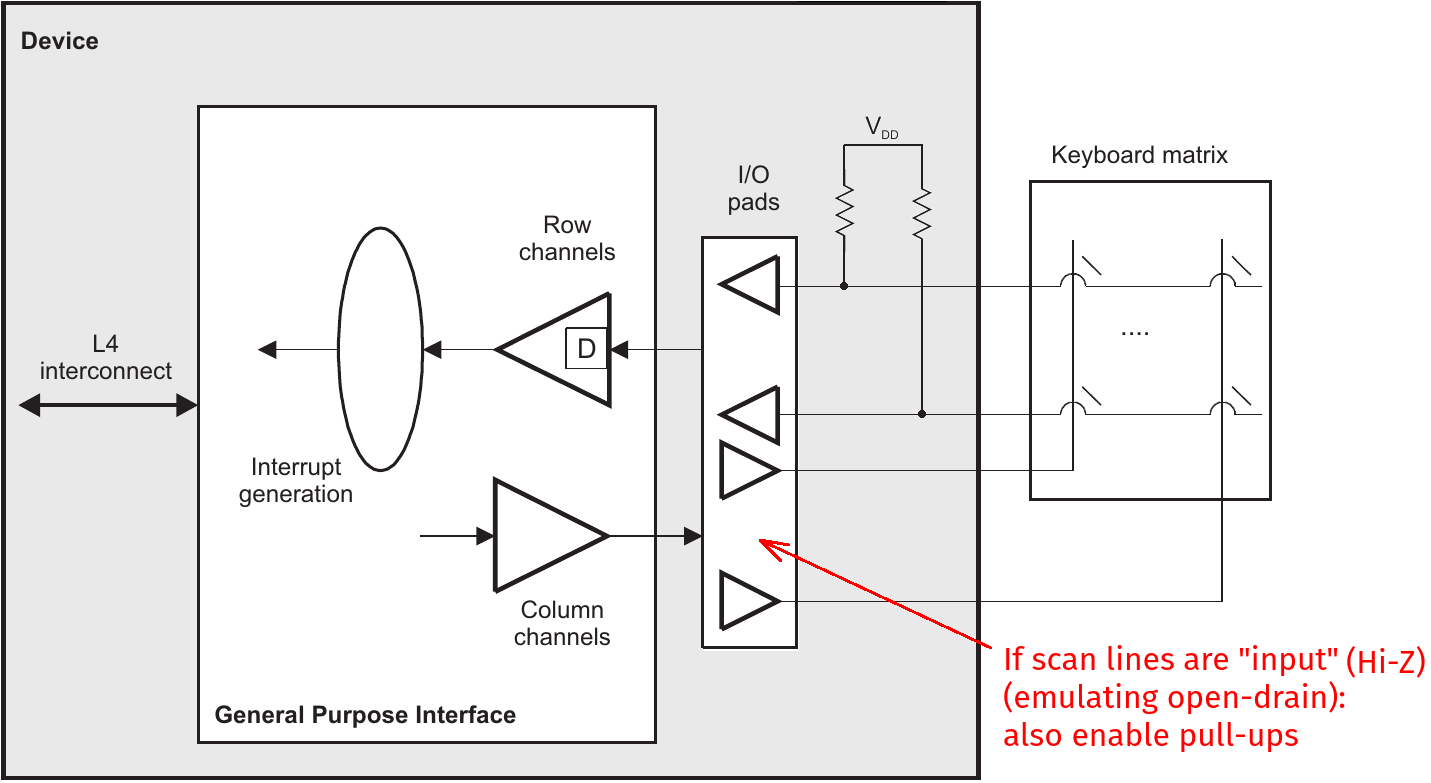
\includegraphics[scale=0.23]{images/keypad-scan2.png}
        \caption{Internal connections}
      \end{figure}
    \column{0.4\textwidth}
      \begin{figure}
        \centering
        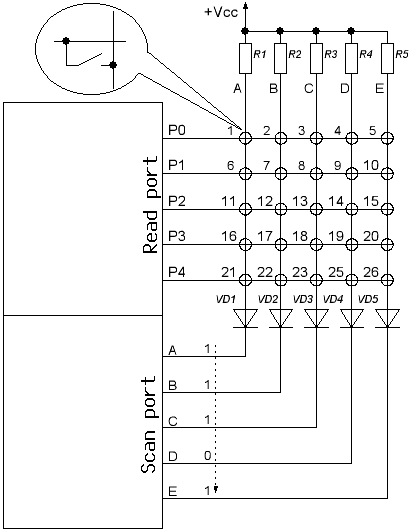
\includegraphics[scale=0.4]{images/keypad-scan1.png}
        \caption{External connections (safe)}
      \end{figure}
  \end{columns}
  \vspace*{-10mm}
\end{frame}

\begin{frame}
  \frametitle{Assignment 2 (cont'd)}
  \begin{columns}
    \column{0.5\textwidth}
      Initialization:
      \begin{itemize}
        \item Pull-up all scan and read lines
        \item Set all scan and read lines into input
        \item Configure debouncing on read lines
      \end{itemize}
      Polling:
      \begin{itemize}
        \item Set all scan lines into input (Hi-Z)
        \item Set one scan line into ``0''
        \item Repeat for next scan line
      \end{itemize}
    \column{0.5\textwidth}
      Scanning (on interrupt):
      \begin{itemize}
        \item Read the state of all read lines
        \item Detect which button was pressed
      \end{itemize}
  \end{columns}
\end{frame}

\begin{frame}
  \frametitle{Assignment 3 (advanced)}
  \begin{itemize}
    \item Find existing driver for matrix keypad in kernel
    \item Find device tree bindings documentation for it
    \item Use this driver instead of your own, make it work
    \item Read and understand that driver's code (especially
          \texttt{input\_dev} API)
  \end{itemize}
\end{frame}

\begin{frame}[standout]
  Thank you!
\end{frame}

\section{Appendixes}

\subsection{Appendix A: Power Management on BBB}

\begin{frame}[standout]
  Appendix A: Power Management on BBB
\end{frame}

\begin{frame}[containsverbatim]
  \frametitle{Appendix A: Power Management on BBB}
  \begin{itemize}
    \item Cortex-M3 core is used as a power supervisor
    \item Make sure your kernel has \texttt{CONFIG\_AMX3\_PM} option
    \item Obtain firmware for Cortex-M3 and copy it to kernel dir:
      \begin{lstlisting}[language=bash,numbers=none]
`\$` git clone git://git.ti.com/processor-firmware/ti-amx3-cm3-pm-firmware.git
`\$` cd ti-amx3-cm3-pm-firmware
`\$` git checkout ti2018.05
`\$` cp bin/am335x-pm-firmware.elf ~/repos/linux-stable/firmware
      \end{lstlisting}
  \end{itemize}
\end{frame}

\begin{frame}[containsverbatim]
  \frametitle{Appendix A: Power Management on BBB (cont'd)}
  \begin{itemize}
    \item Add next options to \texttt{bbb.cfg} fragment and build the kernel:
      \begin{lstlisting}[language=bash,numbers=none]
# --- PM (see sprac74a.pdf) ---
# Embed firmware in kernel
CONFIG_EXTRA_FIRMWARE="am335x-pm-firmware.elf"
CONFIG_EXTRA_FIRMWARE_DIR="firmware"
# AMx3 Power Config Options
CONFIG_MAILBOX=y
CONFIG_OMAP2PLUS_MBOX=y
CONFIG_REMOTEPROC=y
CONFIG_WKUP_M3_RPROC=y
CONFIG_WKUP_M3_IPC=y
CONFIG_SOC_TI=y
CONFIG_TI_EMIF_SRAM=y
CONFIG_AMX3_PM=y
# RTC
CONFIG_RTC_DRV_OMAP=y
      \end{lstlisting}
  \end{itemize}
\end{frame}

\begin{frame}[containsverbatim]
  \frametitle{Appendix A: Power Management on BBB (cont'd)}
  \begin{itemize}
    \item Kernel will upload the firmware to Cortex-M3
    \item Now it's possible to issue PM operations (suspend/resume)
    \item Don't try to load the firmware from user space (using
          \texttt{CONFIG\_FW\_LOADER\_USER\_HELPER*}), mdev doesn't support it
    \item For details see:
          \url{http://www.ti.com/lit/an/sprac74a/sprac74a.pdf}
  \end{itemize}
\end{frame}

\subsection{Appendix B: Device Tree Overlays}

\begin{frame}[standout]
  Appendix B: Device Tree Overlays
\end{frame}

\begin{frame}
  \frametitle{Appendix B: Device Tree Overlays}
  \begin{itemize}
    \item Instead of messing with \texttt{am335x-boneblack.dtb}, it would be
          nice to load Device Tree definitions for external devices
          incrementally
    \item Device Tree Overlays (\texttt{.dtbo}) to the rescue!
    \item \alert{Bad news}: \texttt{CONFIG\_OF\_CONFIGFS} is still not merged
          in kernel, so we can't merge overlays in kernel (via ConfigFS)
    \item \textcolor{green}{Good news}: we still can merge overlays into
          \texttt{dtb} in U-Boot
    \item See \texttt{fdt apply} command in U-Boot shell
  \end{itemize}
\end{frame}

\begin{frame}[containsverbatim,allowframebreaks=1]
  \frametitle{Appendix B: Device Tree Overlays (cont'd)}
  \lstinputlisting[caption=hw3.dtso]{materials/module3/dtbo/hw3.dtso}
\end{frame}

\begin{frame}[containsverbatim]
  \frametitle{Appendix B: Device Tree Overlays (cont'd)}
  Commands to build \texttt{.dtso} \textrightarrow \texttt{.dtbo}
  \begin{lstlisting}[language=bash,numbers=none]
input=hw3.dtso
gen=hw3_gen.dtso
output=hw3.dtbo
kernel_dir=~/repos/linux-stable
gcc_flags="-E -P -x assembler-with-cpp -I$kernel_dir/include -o $gen"
dtc_flags="-W no-unit_address_vs_reg -I dts -O dtb -o $output -b 0 -@"

gcc $gcc_flags $input
dtc $dtc_flags $gen
  \end{lstlisting}
\end{frame}

\end{document}
